\chapter{Tecniche di giunzione}\label{chp:Giunzione}
Prevede di unire più componenti meccanici ne caso in cui non sia possibili ottenere un prodotto finito solo tramite le lavorazioni convenzionali e non convenzionali.
Le principali tecniche sono:
\begin{description}
\item[Fissaggio meccanico]: si tratta di fissaggi non removibili, quindi niente bulloneria piuttosto rivettature.
\item[Saldatura a freddo] Creazione di un legame metallurgico mediante adesione e diffusione.
Viene anche detta saldatura a freddo.
\item[Saldatura a caldo] Unione tramite fusione con l'uso di varie fonti di calore. Detta saldatura a caldo
\item[Brasatura] legami con l'aggiunta di metalli bassofondenti.
\end{description}

La giunzione viene utilizzata perché non siamo in grado di realizzare un prodotto complessivo in un unico colpo ma in successivi assemblaggi.
In genere si parla di giunzioni su metalli, non sono da escludere tecniche su ceramici e polimerici.

\section{Classificazione delle tecniche}
Le principali tecniche di fissaggio sono quelle della figura \ref{fig:Fissaggi}.

\begin{figure}
\centering
\subfloat[][\emph{Principali tecniche di fissaggio}\label{fig:Fissaggi}]
{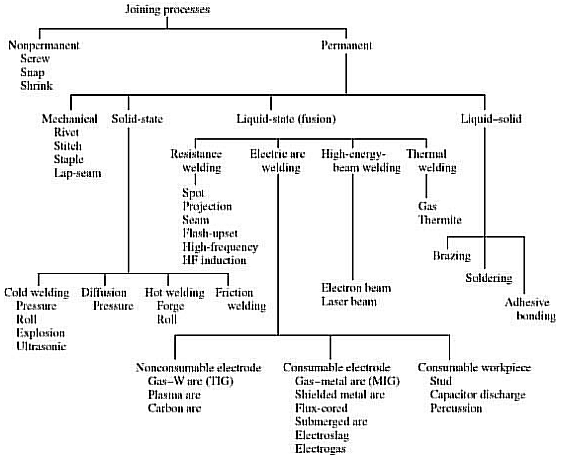
\includegraphics[width = \textwidth]{Fissaggi}}\\
\subfloat[][\emph{Confronto tra le tecniche di fissaggio}\label{fig:ConfFissaggi}]
{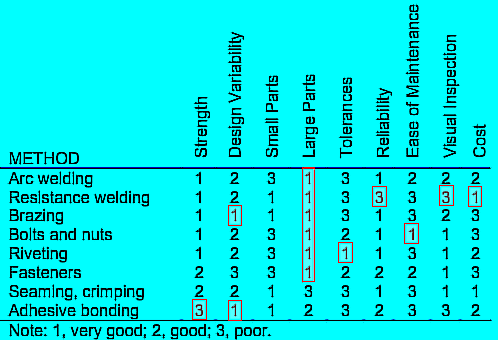
\includegraphics[width = 0.8\textwidth]{ConfFissaggi}}
\caption{Fissaggi}
\label{fig:TipiFissagi}
\end{figure}

Le tecniche di giunzione sono tra le tecniche che maggiormente si tende ad automatizzare.
In genere perché:
\begin{enumerate}
\item Il personale deve essere altamente formato.
\item In particolare per le saldature a caldo possono generarsi dei fumi nocivi o comunque ambienti pericolosi.
\end{enumerate}

\begin{description}
\item[\eng{arc welding}] Si sfrutta un arco elettrico per portare il materiale apportato a fusione.
\item[\eng{Resistence Welding}] la modalità non è diversa dalla precedente ma si sfrutta la legge di Ohm per scaldare il materiale.
\item[Brasatura] Si apporta del materiale bassofondente per legare i componenti.
\item[Bullonatura] Si sfruttano dei componenti meccanici per mantenere uniti più pezzi.
\item[Ritevettatura] Come prima ma non removibile
\item[Grafettatura] Si usano delle graffette per mantenere uniti più componenti.
\item[Aggraffatura] Specifico per lamiere, prevede di utilizzare delle specifiche forme per unire le lamiere, se ne era già parlato quando si è parlato nella piegatura delle lamiere al capitolo \ref{chp:Lamiere} a pagina \pageref{chp:Lamiere}.
\item[Incollaggio] Si utilizza un collante per tenere uniti più pezzi.
\end{description}

\section{Giunzioni meccaniche}
\subsection{Rivettatura}
Si tratta di una giunzione realizzata tramite una specie di chiodo che poi viene opportunamente lavorato per permettergli di mantenere giuntate le componenti, tramite la realizzazione di due teste aderenti ai componenti.
Si chiamano rivetti e alcuni sono mostrati in figura \ref{fig:TipiRivetti}.

\begin{wrapfloat}{figure}{O}{0pt}
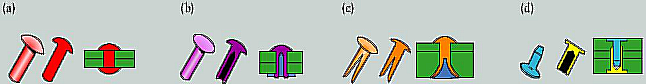
\includegraphics[width = \textwidth, angle = 90]{TipiRivetti}
\caption{Tipologie di rivetti}
\label{fig:TipiRivetti}
\end{wrapfloat}

La più comune tra le rivettature è a \textbf{Rivetti ciechi} come quelli in figura \ref{fig:RivettoCieco}.

\begin{figure}
\centering
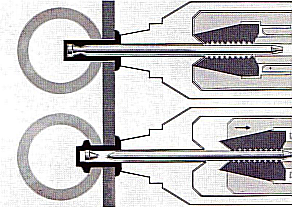
\includegraphics[width = 0.5\textwidth]{RivettoCieco}
\caption{Rivettatura cieca}
\label{fig:RivettoCieco}
\end{figure}

Il fatto che la rivettatura sia costosa rispetto ad altre giunzioni per il fatto che i componenti da giuntare devono già essere forati. Per cui si deve aggiungere una lavorazione aggiuntiva per poter rivettare.
In più la foratura è una fonte di incertezza sul comportamento a fatica del prodotto rivettato.
In più c'è il problema di dover sbavare i fori, in quanto le bave sono fonte di tensioni residue.

\begin{figure}
\centering
\subfloat[][\emph{Rivetto troppo lungo}\label{fig:TooLong}]
{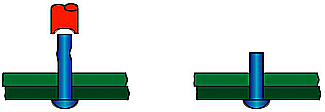
\includegraphics[width = 0.4\textwidth]{TooLong}}\quad
\subfloat[][\emph{Rivetto coperto}\label{fig:Covered}]
{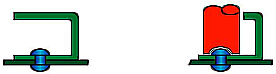
\includegraphics[width = 0.4\textwidth]{Covered}}\\
\subfloat[][\emph{Adesione non completa}\label{fig:NotProperly}]
{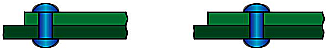
\includegraphics[width = 0.4\textwidth]{NotProperly}}\quad
\subfloat[][\emph{Troppo vicino al bordo}\label{fig:NearEdge}]
{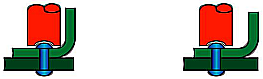
\includegraphics[width = 0.4\textwidth]{NearEdge}}
\caption{Considerazione sulla corretta rivettatura}
\label{fig:ConsRiv}
\end{figure}
I casi che possono portare alla rivettatura a fallire prematuramente possono essere:
scegliere correttamente la dimensione del rivetto perché si rischia di piegare il gambo piuttosto di realizzare la testa, caso \ref{fig:TooLong}.
Bisogna lasciare il giusto spazio affinché la macchina che crea la testa possa lavorare correttamente, caso \ref{fig:Covered}.
Anche il fatto di forare vicino ai bordi può essere fonte di pessimo comportamento a fatica, caso \ref{fig:NearEdge}.

\subsection{Grafettatura}
Si possono realizzare giunzioni tramite una graffetta per lamiere, \ref{fig:Graffettatura}.
Non hanno alti carichi di giunzione ma vengono alle volte usate per la realizzazione di mobili.

\begin{figure}
\centering
\subfloat[][\emph{Esempi di graffettatura}\label{fig:Graffettatura}]
{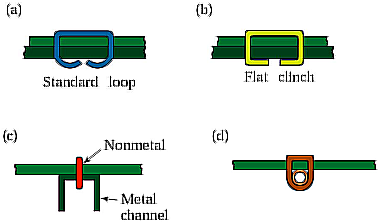
\includegraphics[width = 0.4\textwidth]{Graffettatura}}\:
\subfloat[][\emph{Realizzazione dell'aggraffatura}\label{fig:Aggraffatura}]
{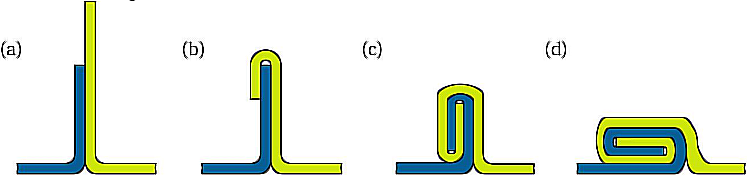
\includegraphics[width = 0.4\textwidth]{Aggraffatura}}\\
\subfloat[][\emph{Esempio di fissaggio \eng{snap-fit}}\label{fig:SnapFit}]
{\includegraphics[width = 0.4\textwidth]{Snapfit}}
\caption{Fissaggi meccanici di graffettatura, aggraffatura e \eng{snap-fit}}
\label{fig:GripMec}
\end{figure}

\subsection{Aggraffatura}
Si era anticipato l'argomento al capitolo \ref{chp:Lamiere} a pagina \pageref{chp:Lamiere}.
Comunque in figura \ref{fig:Aggraffatura} è riproposto il processo per realizzare tale tipo di giunzione.

\subsection{Giunzione a deformazione plastica}
Si realizzano delle piccole deformazioni del materiale per poter alloggiare delle giunzione tra un nucleo e manicotto.
Si possono sfruttare le variazioni dimensionali tramite variazione termica per poter facilitare la giunzione.
È una tecnica particolarmente usata in ambito elettrotecnico per realizzare gli ancoraggi ai morsetti ed eventuali collegamenti tra metalli diversi (tipo rame-alluminio).
Alcuni esempi sono alla figura \ref{fig:DefPlastGrip}.

\begin{figure}
\centering
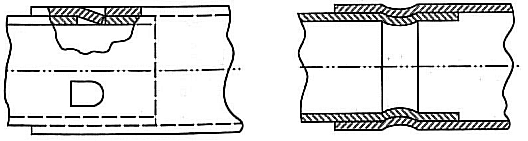
\includegraphics[width = 0.5\textwidth]{DefPlastGrip}
\caption{Alcuni esempi di fissaggio per deformazione plastica}
\label{fig:DefPlastGrip}
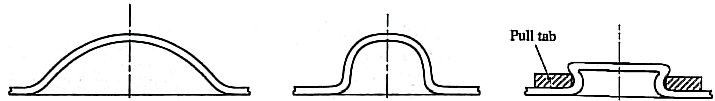
\includegraphics[width = 0.5\textwidth]{Ribattitura}
\caption{Processo di ribattitura}
\label{fig:Ribattitura}
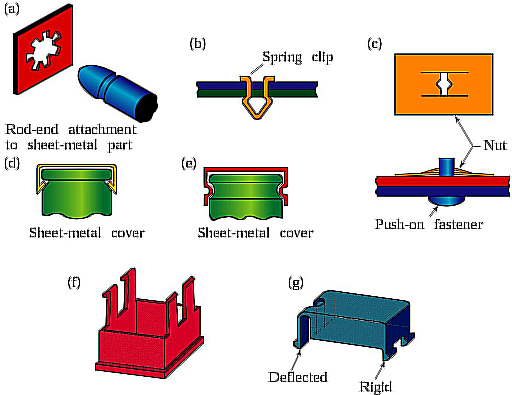
\includegraphics[width = 0.5\textwidth]{AltriGripMec}
\caption{Ulteriori metodi di fissaggio meccanico utilizzati}
\label{fig:AltriGripMec}
\end{figure}

\subsubsection{\eng{Sanp-fit}}
Detta anche chiusura a scatto, \ref{fig:SnapFit}. Viene molto apprezzata per:
\begin{itemize}
\item Basse forze di montaggio,
\item elevate forze di smontaggio,
\item semplici movimenti di montaggio,
\item \eng{feedback} sonoro o tattile,
\item facilità di automazione,
\item assenza di minuteria,
\item omogeneità dei materiali.
\end{itemize}

\subsubsection{Ribattitura}
Si "gonfiano" le lamiere e successivamente viene deformata per poter fissare entrambe tramite la deformazione di entrambe. 
Il processo è riportato alla figura \ref{fig:Ribattitura}.
Viene usata per la realizzazione dell'accoppiamento tra lattina e aprilattina.

Invece, alla figura \ref{fig:AltriGripMec} sono riportati ulteriori metodi di fissaggio meccanico.

\pagebreak


\section{Saldature allo stato solido}
\missingfigure{Tipi saldature a freddo}
DI testa, ad angolo, a T, per sovrapposizione e di spigolo
\todo{\\Elenco}
Vengono realizzate senza portare a fusione il materiale.
La saldatura a freddo svincola dalla necessità di avere dei materiali che hanno temperature di fusione vicine.
Si prenda come esempio il caso di giuntare dei profili di rame con quelli di alluminio per la realizzazione di trasformatori elettrici.

Nella saldatura a freddo non si scalda il materiale, per cui è necessario avere un'ottima preparazione della superficie dei due materiali.
In particolare è opportuno che il substrato di entrambi i materiali deve esser preparato per poter eseguire correttamente la giunzione.
Deve venire a contatto senza che vi sia presenza di ossidi, polveri ecc\dots
Per rimuovere i contaminanti si possono pulire tramite solventi per rimuovere le impurità. Anche spazzolare contribuisce ad aumentare la rugosità superficiale: si aumenta l'estensione della superficie cioè l'area su cui realizzare il legame.
Poi si usa il moto relativo che aiuta a rimuovere eventuali film di ossido.
Applicando la deformazione si deforma plasticamente aprendo il film ossido portando alla luce il substrato duttile.
In teoria non sarebbe necessaria alcuna pressione per effettuare questo tipo di saldature. Viene comunque usata per deformare plasticamente i materiali, facendo in modo che le superfici si conformino l'una all'altra.

Per queste saldature il calore serve per favorire la duttilità dei materiali, facilitando l'intimo contatto dei due substrati.

\paragraph{Saldatura a freddo per sovrapposizione}
Si basa su una forte dilatazione delle superfici.
\missingfigure{saldatura a freddo per sovrapposizione}

Con forti riduzioni di spessore della saldatura a rulli si ottiene una grande espansione della superficie.
Il legame può essere impedito localmente con un distanziale.

\paragraph{Saldatura a freddo di testa}
\paragraph{Saldatura a freddo di profili}
\paragraph{Saldatura a freddo per esplosione}
\paragraph{Saldatura a freddo ad ultrasuoni}
Si erano già anticipati con le lavorazioni non convenzionali
\missingfigure{Ultrasuoni}

\subsection{Saldature per diffusione}
Si potrebbero eseguire anche senza avere temperature eccessivamente alte. Nella pratica vengono comunque sfiorate le temperature normali per favorire la corretta avvenuta della giunzione.
Si era anticipato l'argomento quando si era accennato alla superplasticità.
Si raggiunge tale stato per poter deformare molto semplicemente e a ridotto impiego di forze, dei materiali che risulterebbero decisamente molto duri.
Anche la saldatura per diffusione è un processo molto lento.
Viene usata per realizzare tutti quei materiali placcati d'oro.

Si mette il tutto in un forno, si sovrappone al materiale una foglia d'oro e poi viene applicato un peso per garantire la diffusione.

\missingfigure{Saldature per diffusione}

\section{Saldature a caldo}
Si rifanno direttamente alle lavorazioni per deformazione plastica a caldo già viste in precedenza.
Risulta essere la più antica forma di saldatura per materiali ferrosi.
C'è stata un'evoluzione nella tecnica di di tali la\todo{\\Aggiungi}

Fondamentalmente si può praticamente tutte le tecniche di riscaldamento, L'importante è la successiva pressione da dare ai materiali.
Con questo tipo di saldatura, in trazione si rompe il materiale base non il giunto.

\section{Saldatura a frizione}
Si tratta di una tecnica con cui scaldiamo gli elementi da giuntare.
\missingfigure{Saldatura per frizione}
L'attrito determina il riscaldamento dell'interfaccia in più la pressione simultanea andrà a giuntare i due pezzi. Si forma un colletto di bava
\missingfigure{Processo di saldatura per attrito}
Si presenta un piccolo errore nella figura perché si dovrebbe mettere in rotazione, premere poco.
Poi fermare la rotazione, aumentare la forza in cui si genera anche la bava. 
per poi finire finché la zona pastosa non si raffredda.

\subsection{friction stir welding}
Si tratta di una tecnica che si è sviluppata per la saldatura di teste per lamiere di spessore piuttosto pronunciato. 
Risulta interessante per via del fatto che la macchina necessaria per il raggiungimento dello scopo basta una fresa a controllo numerico.

L'utensile ruota, scalda il materiale delle due lamiere avvicinate, percorre un qualsiasi percorso di saldatura come se fosse una fresa. 